\chapter{Electronic Document Submission}
\label{ap:elect_doc}

The university requires all dissertations and theses to be submitted electronically as 
a PDF document. All required fonts should be embedded in the PDF document to ensure that
your document will appear as intended wherever it is viewed. You can verify that all fonts
are appropriately embedded by opening your PDF document in Adobe Acrobat Reader and selecting
{\ttfamily{File->Properties}}. Under the Font tab, you should see a list of the fonts used in your document.
To ensure that all fonts are embedded, they should be designated as ``Embedded" or ``Embedded 
Subset" in the list.

\section{PDF Bookmarks}
The PDF document must contain bookmarks for preliminary pages plus chapter headings and 
subheadings, as listed in the Table of Contents. In the PDF document, bookmarks should be 
displayed in a panel to the left of the document pages as seen in Figure~\ref{fig:PDF_doc}. 

\begin{figure}[htbp]
\centering
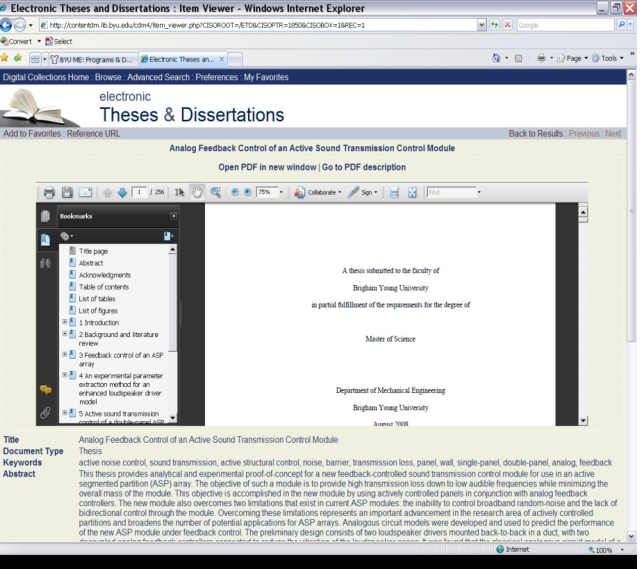
\includegraphics[width=4.5in]{figures/PDF_doc}
\caption{PDF thesis document showing ETD bookmarks.}
\label{fig:PDF_doc}
\end{figure}

If assistance is needed with embedding, bookmarks, or other aspects of submitting the ETD, 
you may obtain assistance at the Multi-media lab in the HBLL. Please note that keywords for 
your research, as listed at the bottom of Figure~\ref{fig:PDF_doc}, will be required at the
time you submit your document. Keywords must be in lower case, unless they are acronyms or 
proper nouns. In addition, a copy of the abstract must be inserted.

Tables and figures appearing in appendices should be numbered A.1, B.1, etc. and should be 
included in the lists of tables and figures.

\section{Miscellaneous Filler}
Most appendices will be longer than 3/4 of a page. We'll use some Latin to fill this one out. {\color{mediumgray} \blindtext}



